\documentclass[hidelinks, a4paper, 12pt]{article}
\usepackage[linktoc=all]{hyperref}
\usepackage{apacite}
\usepackage[margin=1.0in]{geometry}
\usepackage{amssymb}
\usepackage{amsmath}
\usepackage{amsthm}
\newtheorem{theorem}{Theorem}
\usepackage{pgfplots}
\pgfplotsset{compat=1.16}
\usepackage{tikz}
\usepackage{pgf}
\usepackage{mathrsfs}
\usepackage{array}
\usepackage{tabularx}
\usepackage{braket}

\allowdisplaybreaks


\hypersetup{
    pdftitle={Heisenberg Uncertainty Principle},
    pdfauthor={Wilson Wongso},
    pdfpagemode=UseOutlines,
}

\title{Heisenberg Uncertainty Principle}
\author{Notes taken by Wilson Wongso}
\date{}

\setcounter{section}{-1}
\setcounter{tocdepth}{2}

\graphicspath{ {./images/} }

\newcommand{\biimp}{\Leftrightarrow}
\newcommand{\bd}{\textbf}
\newcommand{\n}{\\[\baselineskip]}
\newcommand{\real}{\mathbb{R}}
\newcommand{\thus}{\Rightarrow}
\newcommand{\xhat}{\hat{x}}
\newcommand{\pxhat}{\hat{p}_x}

\begin{document}

    \maketitle
        
    \tableofcontents

    \section{Preface}
        The following notes are based on the lecture video \bd{The Heisenberg Uncertainty Principle: Proof/Explanation} \cite{QM-Heisenberg}.
        The author simply wishes to compile a part of his learning journey into this document.

    \section{Heisenberg Uncertainty Principle}
        Heisenberg Uncertainty Principle states that the more precisely determined a particle's position is, the less precisely is its momentum.
        It is represented by:
        \[\sigma_x \sigma_{p_x} \geq \frac{\hbar}{2}\]
        where $x$ represents position and $p_x$ represents momentum.

    \section{Proof of Heisenberg Uncertainty Principle}
        In order to prove, we must recall several components. Namely the position operator $\xhat$:
        \begin{equation}
            \xhat = x
        \end{equation}
        and the momentum operator $\pxhat$:
        \begin{equation}
            \pxhat = \frac{\hbar}{i}\frac{\partial}{\partial x}
        \end{equation}
        Recall as well the \bd{Generalized Uncertainty Priciple}. If $\hat{A}$ and $\hat{B}$ are two Hermitian Operators, then:
        \begin{equation}
            \sigma_A \sigma_B \geq \frac{1}{2}|\braket{[\hat{A}, \hat{B}]}|
        \end{equation}
        where the commutator $[\hat{A}, \hat{B}] \equiv \hat{A}\hat{B}-\hat{B}\hat{A}$ is a measure of the extent to which $\hat{A}$ and $\hat{B}$ commutes.
        \begin{theorem}
            Heisenberg Uncertainty Principle
            \[\sigma_x \sigma_{p_x} \geq \frac{\hbar}{2}\]
        \end{theorem}
        \begin{proof}
            We begin by applying Generalized Uncertainty Principle $(3)$ to the position and momentum operators $(1)$ and $(2)$:
            \begin{equation}
                \sigma_x \sigma_{p_x} \geq \frac{1}{2}|\braket{[\xhat, \pxhat]}|
            \end{equation}
            From which we need to evaluate the commutator $[\xhat, \pxhat]$. We can apply the operators to a dummy vector $f$:
            \[\begin{split}
                [\xhat, \pxhat]f &= \xhat(\pxhat f) - \pxhat(\xhat f)\\
                \\
                [\xhat, \pxhat]f &= x\left(\frac{\hbar}{i}\frac{\partial}{\partial x}(f)\right) - \frac{\hbar}{i}\frac{\partial}{\partial x}(xf)\\
                \\
                [\xhat, \pxhat]f &= x\frac{\hbar}{i}\frac{\partial f}{\partial x} - \frac{\hbar}{i}\left(x\frac{\partial f}{\partial x} + f\frac{\partial x}{\partial x}\right)\\
                \\
                [\xhat, \pxhat]f &= -\frac{\hbar}{i}f\\
                \\
                [\xhat, \pxhat]f &= i \hbar f                
            \end{split}\]
            Obtaining that the commutator is given by:
            \begin{equation}
                [\xhat, \pxhat] = i \hbar
            \end{equation}
            Applying $(5)$ to $(4)$:
            \[\begin{split}
                \sigma_x \sigma_{p_x} &\geq \frac{1}{2}|\braket{i \hbar}|\\
                \\
                \sigma_x \sigma_{p_x} &\geq \frac{1}{2}|i \hbar|\\
                \\
                \sigma_x \sigma_{p_x} &\geq \frac{\hbar}{2}
            \end{split}\]
        \end{proof}
    
    \section{Pure Particle and Pure Wave}
        A pure particle's position is well defined, unlike its momentum. On the other hand, a pure wave's momentum is well defined, and its position is poorly defined. We can 
        see it by observing how their wavefunctions are respectively.\n
        Recall that we can relate a particle's momentum $p$ to its wavelength $\lambda$ by de Broglie formula:
        \[p = \frac{2\pi \hbar}{\lambda}\]

        \subsection{Wavefunction of Pure Particle}
            \begin{tikzpicture}
                \begin{axis}[
                    axis lines=middle,
                    xlabel=$x$, xlabel style={at=(current axis.right of origin), anchor=west},
                    ylabel=$\psi$, ylabel style={at=(current axis.above origin), anchor=south},
                    xtick=\empty, ytick=\empty,
                    clip=false,
                ]
                \addplot [
                    domain=0.5:3.1, 
                    samples=100, 
                    color=white,
                ]
                {sin(deg(x))};
                \addplot [
                    domain=1.58:1.6, 
                    samples=100, 
                    color=blue,
                ]
                {50*x-79};
                \addplot [
                    domain=1.6:1.62, 
                    samples=100, 
                    color=blue,
                ]
                {-50*x+81};
                \node[label={90:{particle}},circle,fill,inner sep=2pt] at (axis cs:1.6, 1.05) {};
                \end{axis}
            \end{tikzpicture}\n
            The wavefunction of a pure particle has its position well-defined, hence making $\sigma_x$ \bd{small}. However, since its wavefunction is like a delta-fuction,
            its wavelength is poorly defined, thus $\sigma_{p_x}$ is \bd{large}.

        \subsection{Wavefunction of Pure Wave}
            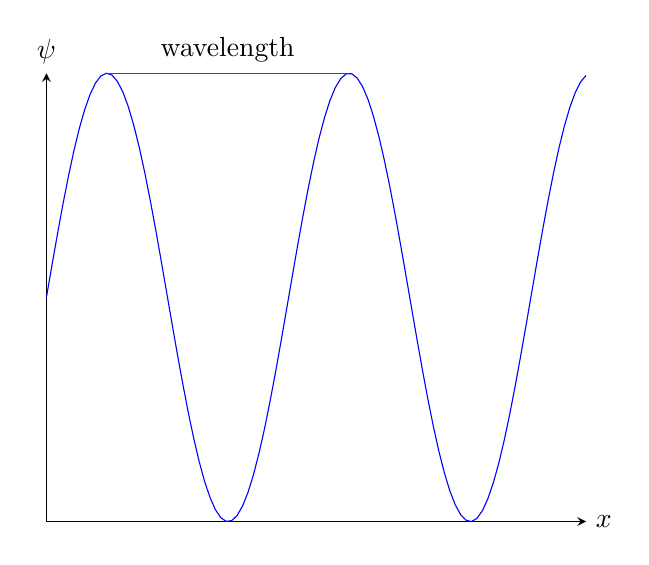
\begin{tikzpicture}
                \begin{axis}[
                    axis lines=middle,
                    xlabel=$x$, xlabel style={at=(current axis.right of origin), anchor=west},
                    ylabel=$\psi$, ylabel style={at=(current axis.above origin), anchor=south},
                    xtick=\empty, ytick=\empty,
                    clip=false,
                ]
                \addplot [
                    domain=0:14, 
                    samples=100, 
                    color=blue,
                ]
                {sin(deg(x)) + 10};
                \addplot [
                    domain=1.57:7.85, 
                    samples=100, 
                    color=red,
                ]
                {11};
                \node[label={90:{wavelength}},circle,inner sep=0.0pt] at (axis cs:4.7, 11) {};
                \end{axis}
            \end{tikzpicture}\n
            Unlike pure particle, the wavelength of a pure wave is well defined, making $\sigma_{p_x}$ \bd{small}. However, its position is poorly defined, making $\sigma_x$ \bd{large}.\n
            These characteristics are inline with the Heisenberg Uncertainty Principle.

    \section{Wavefunction in Position Space and in Momentum Space}
        The wavefunction in position space,
        \[\Psi(x, t)\]
        can be used to determine the probability that a particle's position lies between $x=a$ and $x=b$.\n
        While the wavefunction in momentum space,
        \[\Phi(p, t)\]
        can be used to find the probability that a particle's momentum lies between $p=p_a$ and $p=p_b$.\n
        To obtain $\Phi(p,t)$ from $\Psi(x, t)$, we can utilize \bd{Fourier Transform}, and \bd{Inverse Fourier Transform} for its reverse.\n
        If, in position space, the particle's position is well defined, i.e. $\sigma_x$ is small; in momentum space, $\sigma_{p_x}$ is large:\n
        \begin{tikzpicture}
            \begin{axis}[
                axis lines=middle,
                xlabel=$x$, xlabel style={at=(current axis.right of origin), anchor=west},
                ylabel=$\Psi$, ylabel style={at=(current axis.above origin), anchor=south},
                xtick=\empty, ytick=\empty,
                clip=false,
            ]
            \addplot [
                domain=0.5:3.1, 
                samples=100, 
                color=white,
            ]
            {sin(deg(x))};
            \addplot [
                domain=1.58:1.6, 
                samples=100, 
                color=blue,
            ]
            {50*x-79};
            \addplot [
                domain=1.6:1.62, 
                samples=100, 
                color=blue,
            ]
            {-50*x+81};
            \end{axis}
        \end{tikzpicture}
        \begin{tikzpicture}
            \begin{axis}[
                axis lines=middle,
                xlabel=$x$, xlabel style={at=(current axis.right of origin), anchor=west},
                ylabel=$\Phi$, ylabel style={at=(current axis.above origin), anchor=south},
                xtick=\empty, ytick=\empty,
                clip=false,
            ]
            \addplot [
                domain=0:14, 
                samples=100, 
                color=blue,
            ]
            {sin(deg(x)) + 10};
            \end{axis}
        \end{tikzpicture}\n
        Similarly, if in momentum space, the particle's momentum is well defined, $\sigma_{p_{x}}$ is small; in position space, $\sigma_x$ is large:\n
        \begin{tikzpicture}
            \begin{axis}[
                axis lines=middle,
                xlabel=$x$, xlabel style={at=(current axis.right of origin), anchor=west},
                ylabel=$\Phi$, ylabel style={at=(current axis.above origin), anchor=south},
                xtick=\empty, ytick=\empty,
                clip=false,
            ]
            \addplot [
                domain=0.5:3.1, 
                samples=100, 
                color=white,
            ]
            {sin(deg(x))};
            \addplot [
                domain=1.58:1.6, 
                samples=100, 
                color=blue,
            ]
            {50*x-79};
            \addplot [
                domain=1.6:1.62, 
                samples=100, 
                color=blue,
            ]
            {-50*x+81};
            \end{axis}
        \end{tikzpicture}
        \begin{tikzpicture}
            \begin{axis}[
                axis lines=middle,
                xlabel=$x$, xlabel style={at=(current axis.right of origin), anchor=west},
                ylabel=$\Psi$, ylabel style={at=(current axis.above origin), anchor=south},
                xtick=\empty, ytick=\empty,
                clip=false,
            ]
            \addplot [
                domain=0:14, 
                samples=100, 
                color=blue,
            ]
            {sin(deg(x)) + 10};
            \end{axis}
        \end{tikzpicture}

    \section{Misconception: Observer Effect}
        Often, the observer effect is mistaken for Heisenberg Uncertainty Principle, for example:\n
        If we want to measure the position of an electron accurately, we need to shine lots of very high-energy light obtaining its accurate position $x$.\n
        However, shining lots of high-energy light will also excite the electron, disabling us from measuring its momentum $p_x$ accurately.
        \[\sigma_{x_{meas}} \uparrow\]
        \[\sigma_{p_{meas}} \downarrow\]
        If we shine very little light, the electron probably won't get excited and we are able to measure its momentum $p_x$ accurately.\n
        Because there is hardly any light, we can't measure its position $x$ accurately.
        \[\sigma_{p_{meas}} \uparrow\]
        \[\sigma_{x_{meas}} \downarrow\]
        However, this is not the Heisenberg Uncertainty Principle! Heisenberg Uncertainty Principle is not a statement about our inability to measure things precisely.\n
        Rather, it is a consequence of Mathematics, and it doesn't mention anything about measurements.
    \bibliographystyle{apacite}
    \bibliography{References}

\end{document}